\chapter{Systematic analysis on radial profiles of broadband contribution} \label{ch:EBB}
\graphicspath{{chapter5_ys/}}
\minitoc

In this chapter, a systematic study is carried out of the properties of the frequency spectra from fluctuation measurements using the turbulence database built at Tore Supra. Specifically, we focus on the radial profiles of the broadband contribution ($E_\mathrm{BB}$) of the spectra. Section \ref{sec:radial_profile_OH} presents a number of systematic trends of the database observations of $E_\mathrm{BB}$ in Ohmic plasmas, followed by a deeper discussion in the linear Ohmic confinement (LOC) regime and in the saturated Ohmic confinement (SOC) regime in section \ref{sec:EBB_LOC_SOC}. Section \ref{sec:radial_profile_ICRH_LH} extends the study to the case of plasmas with auxiliary heating, either pure ICRH or LH. It should be noted that all results discussed in this thesis are restricted to the L-mode case, as H-mode was never obtained in Tore Supra discharges. In section \ref{sec:EBB2dn}, additional interpretation is given of $E_\mathrm{BB}$ and a link between $E_\mathrm{BB}$ and the turbulence level ($\delta n/n$) is established. Summary and discussion are given in section \ref{summary_discussion}.


\section{General trends of $E_\mathrm{BB}$ in Ohmic plasmas} \label{sec:radial_profile_OH}

We first investigate the spectrum properties in Ohmic plasmas. Recalling the discussion in section \ref{sec:Criteria_parameter}, only the frequency spectra with low noise level (SNR $>$ 25 dB), dominated by perpendicular reflection (Doppler shift $<$ 50 kHz) in stationary state ($I_p =$ constant during the acquisition time) are considered in the statistical analysis. Our operational definition of an Ohmic plasma covers all cases where each source of auxiliary heating power is below 0.1 MW. For Tore Supra, this means that $P_{ICRH} < 0.1$ MW, $P_{LH} < 0.1$ MW and $P_{ECRH} < 0.1$ MW. This constraint results in a data set consisting of $\sim$ 180,000 spectra from nearly 3,000 discharges. The data set covers the entire radial range from the LFS to the HFS.


\subsection{$E_\mathrm{BB}$ profiles at varying $q_{\psi}$}


%%%%%%%%%%%%%%%%%%%%
\begin{figure}[h]
\begin{centering}
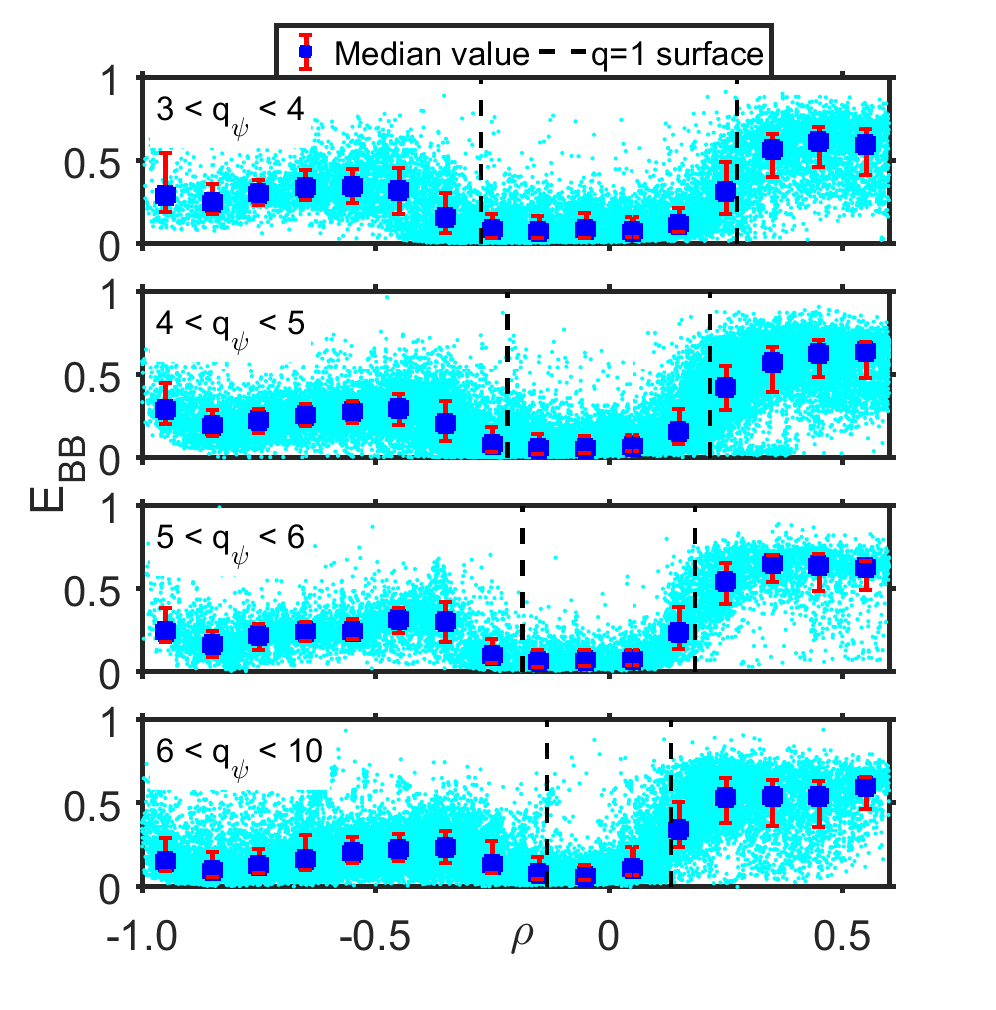
\includegraphics[scale=0.6]{fig_EBB_OH.eps}
\par\end{centering}
\caption{Radial profiles of $E_\mathrm{BB}$ for different $q_{\psi}$ as a function of normalized radius $\rho = rcos(\theta)/a$, where $a$ is the minor radius of the tokamak ($a \sim 0.72$ m for Tore Supra). Negative ($\theta = 2\pi$) and positive ($\theta = 0$) values refer to the HFS and LFS, respectively. The cyan points are obtained from the individual fitted spectra. The blue square points denote median values calculated within small radial intervals ($\delta\rho \sim 0.1$), with red error bars around the median given by the mean absolute deviation. The $q = 1$ positions are indicated by the black dashed lines.}
\label{fig:EBBOhmic}
\end{figure}
%%%%%%%%%%%%%%%%%%%%

We have investigated the relation between $E_\mathrm{BB}$ obtained from the parametrization and various dimensionless quantities determining the confinement performance. We consider radial profiles of $E_\mathrm{BB}$ for varying edge safety factor ($q_{\psi}$), as shown in figure \ref{fig:EBBOhmic}. The most remarkable feature is a clear reduction of $E_\mathrm{BB}$, which we refer to as the \emph{energy basin}, in the core region for all ranges of $q_{\psi}$. Furthermore, there is a clear asymmetry between the HFS and LFS: $E_\mathrm{BB}$ tends to slowly increase from the inner edge (Lorentzian spectra) towards the center up to the cliff (Gaussian spectra) before the energy basin on the HFS, whereas on the LFS $E_\mathrm{BB}$ is much higher and reaches saturation (wide Gaussian spectra) above $E_{BB} > 0.5$, indicating that the BB component prevails in the reflected spectra.


%%%%%%%%%%%%%%%%%%%%
\begin{figure}[h]
\begin{centering}
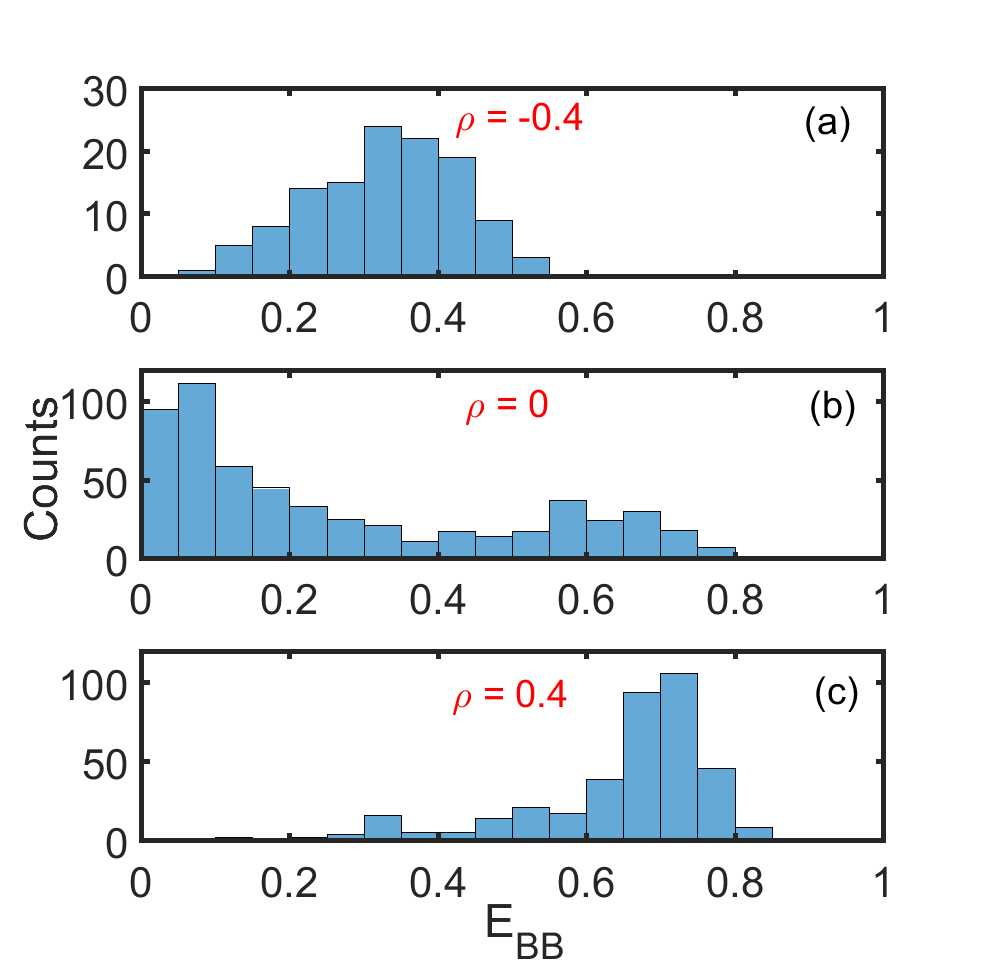
\includegraphics[scale=0.62]{fig_HistEBB.eps}
\par\end{centering}
\caption{Different distributions of $E_\mathrm{BB}$ at fixed radial positions: (a) $\rho = -0.4$, (b) $\rho = 0$, (c) $\rho = 0.4$, under the condition $5 < q_{\psi} < 6$.}
\label{fig:HistEBB}
\end{figure}
%%%%%%%%%%%%%%%%%%%%


The considerable radial variation of $E_\mathrm{BB}$ is not possible caused by the finite beam width, which is expected to be larger than the BB turbulence wavelength. On the other hand, the wavelength of the LF component can be longer than the beam width at the edge, while approaching the beam width close to the center. Unfortunately, Doppler reflectometry, which can evaluate the poloidal correlation length, is not available for core and HFS measurements. However, if the beam size effects were predominant, one would neither observe a change of the position of the energy basin with varying edge $q$, nor the rise of the $E_\mathrm{BB}$ on the HFS from the edge up to the basin cliff.

Furthermore, figure \ref{fig:EBBOhmic} shows that, at fixed radial position, $E_\mathrm{BB}$ still varies considerably across the database, for all values of $q_{\psi}$. This can be attributed to fitting errors and varying global operational conditions. In Figure \ref{fig:HistEBB}, the distributions of $E_\mathrm{BB}$ are shown at three radial positions ($\rho = -0.4, 0, 0.4$), in the range $5 < q_{\psi} < 6$, where the variance of $E_\mathrm{BB}$ is the lowest. Apart from the large scatter of $E_\mathrm{BB}$ at fixed radial position, differences in the mean and shape of the distributions are also apparent. Because of the non-zero skewness and outliers in the distributions, we use the median of the distribution rather than the mean for systematic studies of the typical $E_\mathrm{BB}$. When calculating this within small radial intervals of width $\sim 0.1$, we obtain the blue squares in figure \ref{fig:EBBOhmic}. The red error bars are given by the mean absolute deviation around the median values within each interval. A similar analysis method relying on the median will be used to capture trends from the highly scattered data hereafter.


\subsection{Relationship between the $E_\mathrm{BB}$ basin and the $q = 1$ surface}

In figure \ref{fig:EBBOhmic}, it can also be seen that, as $q_{\psi}$ increases, the energy basis shrinks. This suggests a relation between the $E_\mathrm{BB}$ basin and the $q = 1$ surface. However, at Tore Supra, systematic derivation of the $q = 1$ surface from the routine equilibrium reconstruction is affected by considerable uncertainties. Another method to obtain the $q = 1$ position can be the analysis of sawteeth instability from ECE electron temperature measurements. Then, the position of the sawteeth inversion indicates the $q = 1$ position. However, the latter method is only feasible for limited discharges but turns out to be difficult for a large database. Therefore, the position was estimated through the approximate empirical relation $\rho_{q=1} = 1/q_{\psi}$, established earlier for TFTR and TFR \cite{Arunasalam_1990_NF}. To verify this relation for our database, we employed several typical discharges at different toroidal magnetic field $B_{0}$ ($3.4$ T and $3.86$ T), as well as a pulse with an $I_{p}$ scan, as shown in figure \ref{fig:rq1}. Here, the $q = 1$ positions of some selected discharges were obtained from the ECE method. These results are consistent with the empirical relation at both low (3.4 T) and high (3.86 T) magnetic fields, only at very high magnetic fields (3.88 T) there exists some differences. Notice that the consistency between the two methods is better at low $q$ when $\rho_{q=1}$ changes with $q$ rapidly, whereas at high $q$ the effects of the uncertainties are limited due to a slow change rate of $\rho_{q=1}$ with $q$. This confirms the validity of this empirical relation and providing a practical means to derive the position of the $q = 1$ surface. In each $q_{\psi}$ range, the median value using $\rho = 1/q_{\psi}$ gives an approximation to the position of the $q = 1$ surface, shown as the two vertical dashed lines in figure \ref{fig:EBBOhmic}.

%%%%%%%%%%%%%%%%%%%%
\begin{figure}[h]
\begin{centering}
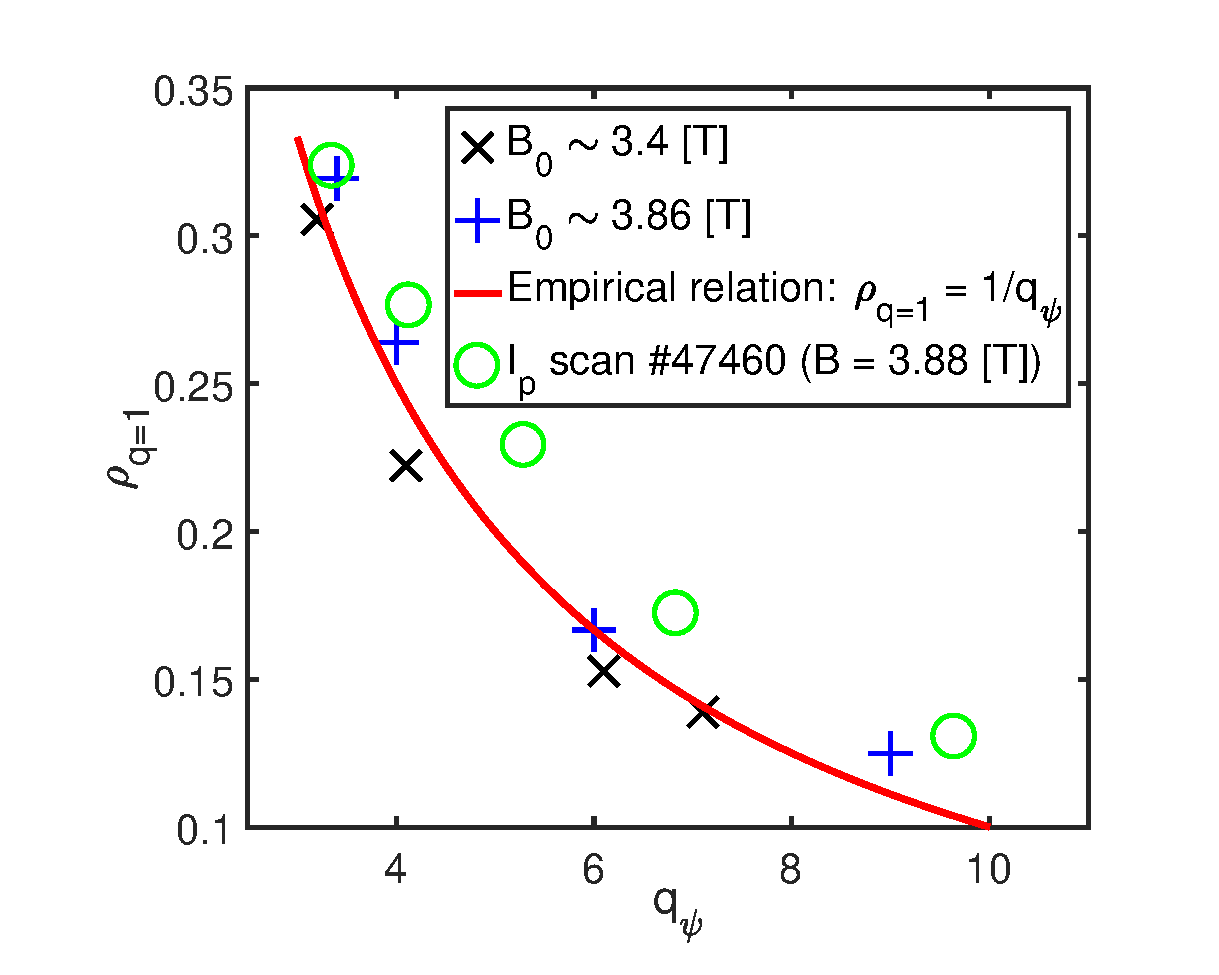
\includegraphics[scale=0.45]{fig_rq1.eps}
\par\end{centering}
\caption{Verification of the empirical relation $\rho_{q=1}=1/q_{\psi}$ by means of a number of typical discharges from the Tore Supra database.}
\label{fig:rq1}
\end{figure}
%%%%%%%%%%%%%%%%%%%%


For a quantitative definition of the width of the $E_\mathrm{BB}$ basin, we employ the criterion $E_{BB}<0.1$ (value of the median). The radial region of the basin and its width ($w$) are indicated by the shaded area and the double arrow shown in figure \ref{fig:EBBOhmic}. In addition, the half-width of the basin ($w$/2) is shown as a function of the normalized $q = 1$ position ($\rho_{q=1}$) in figure \ref{fig:BasinWidth} (a). There is a clear one-to-one correspondence, supporting our hypothesis that the occurrence of the $E_\mathrm{BB}$ basin is related to the $q = 1$ surface. The error bars on the half-width originate from the limitation on the spatial resolution due to the finite number of points in each radial interval.

Furthermore, Figure \ref{fig:BasinWidth} (b) shows the width of the $E_\mathrm{BB}$ basin at the HFS ($\rho < 0$) and LFS ($\rho > 0$) separately. Here, the sum of the basin width at the HFS ($w_\mathrm{HFS}$) and LFS ($w_\mathrm{LFS}$) is just the total basin width ($w$): $w_{HFS}+w_{LFS}=w$. From figure \ref{fig:BasinWidth} (b), it can be seen that both $w_\mathrm{HFS}$ and $w_\mathrm{LFS}$ follow the same increasing trend with respect to $\rho_{q=1}$ as the total width $w$ shown in figure \ref{fig:BasinWidth} (a). However, $w_\mathrm{HFS}$ is systematically higher (2--3 times) than $w_\mathrm{LFS}$, revealing a strong asymmetry of the basin structure at the HFS and LFS. In addition, $w_\mathrm{LFS}$ increases faster than $w_\mathrm{HFS}$ with respect to $\rho_{q=1}$. In other words, the absolute difference between $w_\mathrm{HFS}$ and $w_\mathrm{LFS}$ decreases with increasing $\rho_{q=1}$ (or decreasing $q_{\psi}$).


%%%%%%%%%%%%%%%%%%%%
\begin{figure}[!h]
\begin{centering}
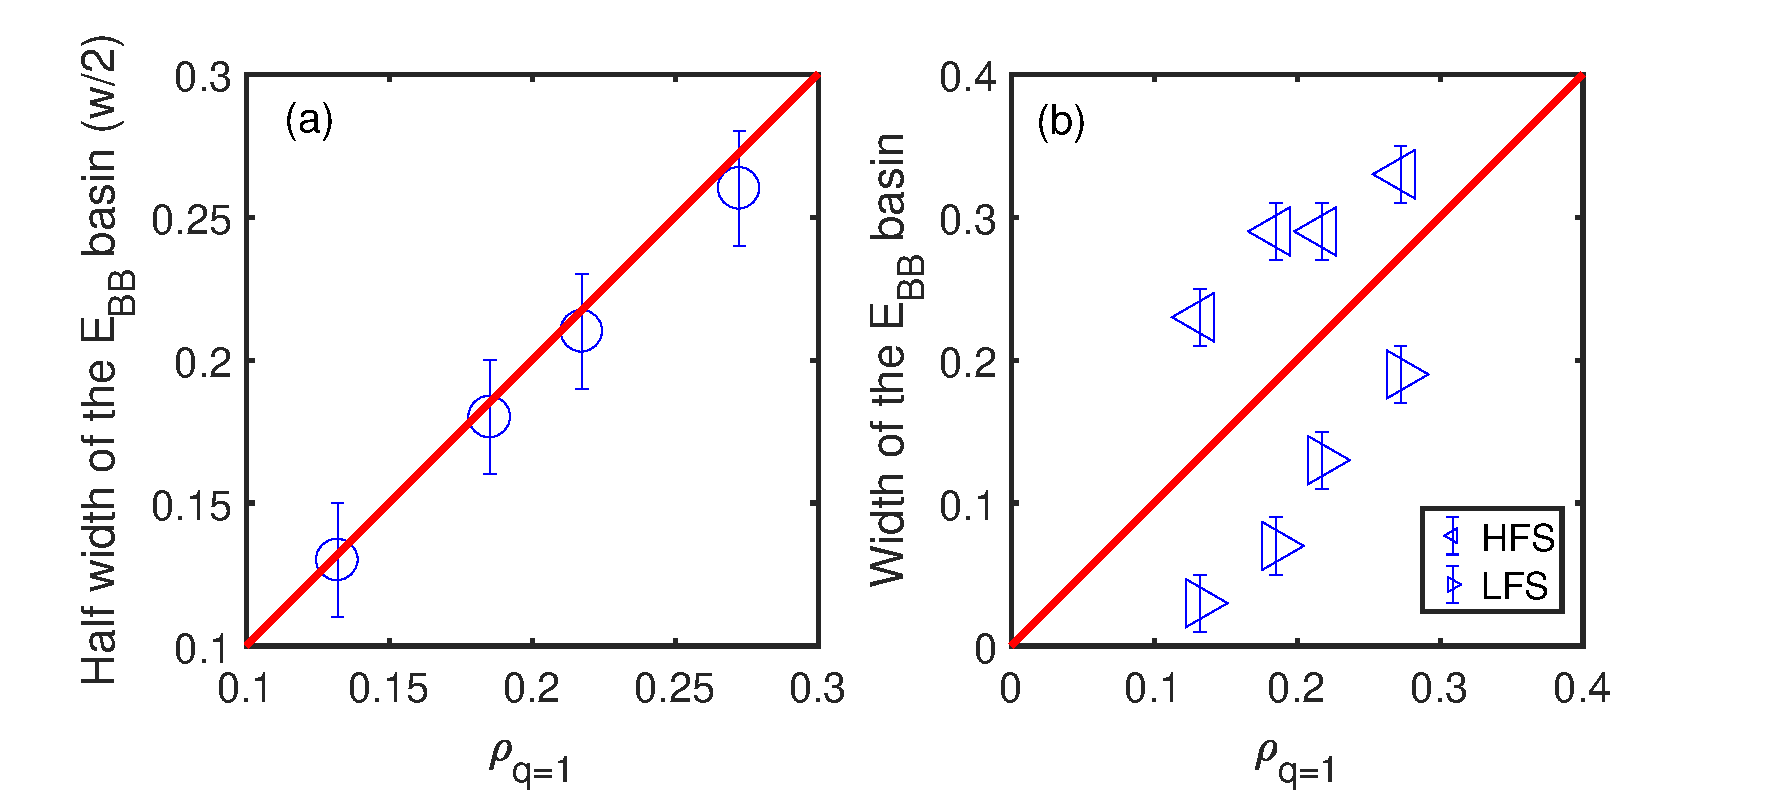
\includegraphics[scale=0.5]{fig_BasinWidth_v2.eps}
\par\end{centering}
\caption{(a) Half-width of $E_\mathrm{BB}$ basin and (b) width of the $E_\mathrm{BB}$ basin at the HFS and LFS as a function of the $q = 1$ position, both values normalized to the minor radius.}
\label{fig:BasinWidth}
\end{figure}
%%%%%%%%%%%%%%%%%%%%


\subsection{Shift of the cutoff layer} \label{sec:shift_of_cutoff}

The strong asymmetry of the $E_\mathrm{BB}$ basin ($w_{HFS} > w_{LFS}$) shown in figure \ref{fig:BasinWidth} (b), can be viewed as a systematic shift towards the HFS of the radial positions. This shift is also observed in figure \ref{fig:EBBOhmic}, where the actual position of the boundaries of the basin do not coincide with the location of the $q = 1$ surface, indicated by the shaded basin region.

In order to understand the origin of this shift, it is important to recall that the radial positions are the probing wave cutoff positions calculated using the density profile from the interferometry diagnostic. Hence, the shift might be due to uncertainties on the density profiles from interferometry. To resolve the matter, we have investigated several tens of Ohmic discharges with available core reflectometry profiles. Usually, interferometry underestimates the core density compared to reflectometry. This can be due to the density plateau and the complicated profile structures near the magnetic axis \cite{Sabot_2006_PPCF}.

%%%%%%%%%%%%%%%%%%%%
\begin{figure}[h]
\begin{centering}
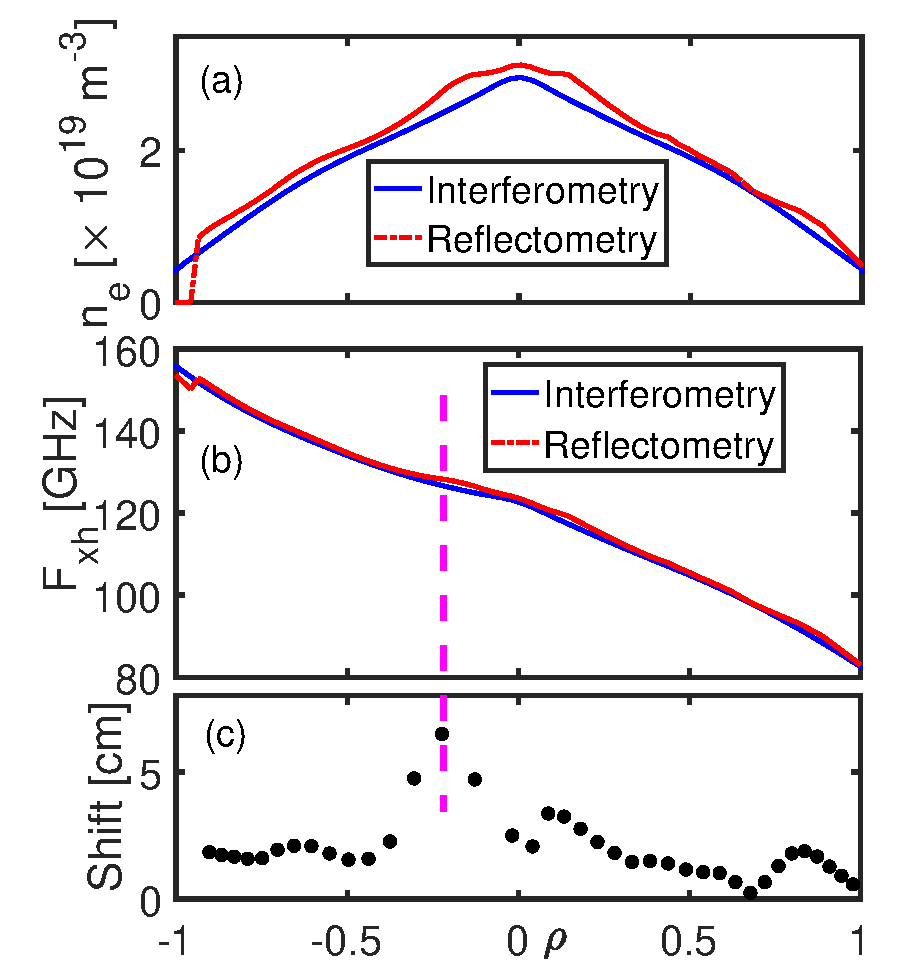
\includegraphics[scale=0.67]{fig_Shift.eps}
\par\end{centering}
\caption{(a) Density profiles and (b) upper cutoff frequencies ($F_{xh}$) near the turbulence signal
obtained by core reflectometry and interferometry. (c) Difference of the cutoff positions from interferometry with respect to reflectometry at different radial positions.}
\label{fig:Shift}
\end{figure}
%%%%%%%%%%%%%%%%%%%%


To illustrate the uncertainties from interferometry and the resulting cutoff shift, Figure \ref{fig:Shift} (a) shows the density profiles from core reflectometry and interferometry, acquired at the same time in one typical discharge. It can be seen that the core density from interferometry is lower than that from reflectometry. We next calculated the cutoff position using each of the two density profiles, confirming a shift towards the HFS of the cutoff layers from interferometry with respect to reflectometry, as plotted in figure \ref{fig:Shift} (c). There is a clear asymmetry, with a much larger shift in the region $-0.3\lesssim\rho\lesssim-0.1$ compared to $0.1\lesssim\rho\lesssim0.3$, i.e. in the vicinity of the $q = 1$ surface. This is consistent with the observation in figure \ref{fig:EBBOhmic}, where the $q = 1$ surface is outside the $E_\mathrm{BB}$ basin on the LFS, but inside the basin on the HFS, with an asymmetry due to the larger shift. The strong shift at the HFS region is caused by the slower increase of the cutoff frequencies (Figure \ref{fig:Shift} (b)) at the HFS than at the LFS \cite{Mazzucato_1998_RSI}. The change of shift is relatively large, even with only a small change of the probing frequency, since the evolution of X-mode upper cutoff frequency with $\rho$ becomes flatter at the HFS, due to the fact that the magnetic field intensity continues to increase, while the density gradient changes sign across the magnetic axis. Thus, the peak of the shift in figure \ref{fig:Shift} (c) corresponds to the flattest part of the cutoff frequency profile deduced from the reflectometry density profile, as indicated by the vertical dashed line in figure \ref{fig:Shift} (b) and (c).

Although the correction of the cutoff shift is feasible for a limited number of selected cases, it is impossible to apply it to a large database with thousands of discharges, as reflectometry density profile measurements cannot be taken at the same time as density fluctuation measurements (as mentioned Section \ref{sec:drefluc}). Nevertheless, the systematic shift should not considerably affect both qualitative observations and quantitative analysis in this work, although it should be kept in mind. However, the systematic shift attributed to uncertainties of interferometry shows the detection limit of general trends using a database study. Put differently, any observed patterns in the data could be the result of database artifacts, and should be verified by a traditional shot-to-shot analysis. On the other hand, such patterns could be a useful indication of systematic errors in any of the involved diagnostic measurements.


\section{Radial profiles of $E_\mathrm{BB}$ in LOC and SOC regimes} \label{sec:EBB_LOC_SOC}


As mentioned in section \ref{sec:confine_regime}, the Ohmic heating plasmas could be further divided into the LOC and SOC confinement regimes. In the LOC regime, the energy confinement time increases with the density at low density. After a density threshold, the confinement becomes the SOC regime where the confinement times does not change with the density. Since the confinement time is directly linked to the turbulence properties, in this section we investigate in what way the change of the confinement regime could affect the broadband contribution $E_\mathrm{BB}$.


\subsection{Separation of LOC and SOC regimes}

In the first step, an effective separation of the LOC and SOC regimes for the Tore Supra database is required. The separation relies on the density threshold of the LOC-SOC transition, which can be approximated as \cite{shimomura_LOC_SOC_transition_1985}:%
%%%%%%%%%%%%%%%%%%%%
\begin{equation}\label{eq:nLOCSOC}
n_\mathrm{LOC-SOC} \approx \frac{5I_p\mu_0}{{\pi}a^2}\sqrt{\frac{A_i\kappa}{2}}.
\end{equation}
%%%%%%%%%%%%%%%%%%%%
\noindent Here, $n_\mathrm{LOC-SOC}$ is the central line-averaged density in $10^{19}$ m$^{-3}$, $I_p$ (A) the plasma current, $a$ (m) the minor radius, $A_i$ the atomic mass number and $\kappa$ the elongation. A previous study based on a number of dedicated Tore Supra discharges \cite{Arnichand_2014_NF} shows that \eqref{eq:nLOCSOC} tends to overestimate the density threshold of the LOC-SOC transition. However, for Tore Supra, all prediction parameters in the scaling \eqref{eq:nLOCSOC} except $I_p$ are almost constant. Specifically, Tore Supra had a circular cross-section and operated with a bottom limiter at an almost constant vertical position, ensuring $\kappa\approx 1$ and $a\approx 0.72$ m. Both $\kappa$ and $a$ have uncertainties less than 5\%. With deuterium operation the atomic mass number $A_i$ is 2, while impurity concentrations were limited, usually less than 10\%. Therefore, we have established a reduced empirical scaling law for $n_\mathrm{LOC-SOC}$ in terms of $I_p$ from a large number of discharges.


%%%%%%%%%%%%%%%%%%%%
\begin{figure}[h]
\begin{centering}
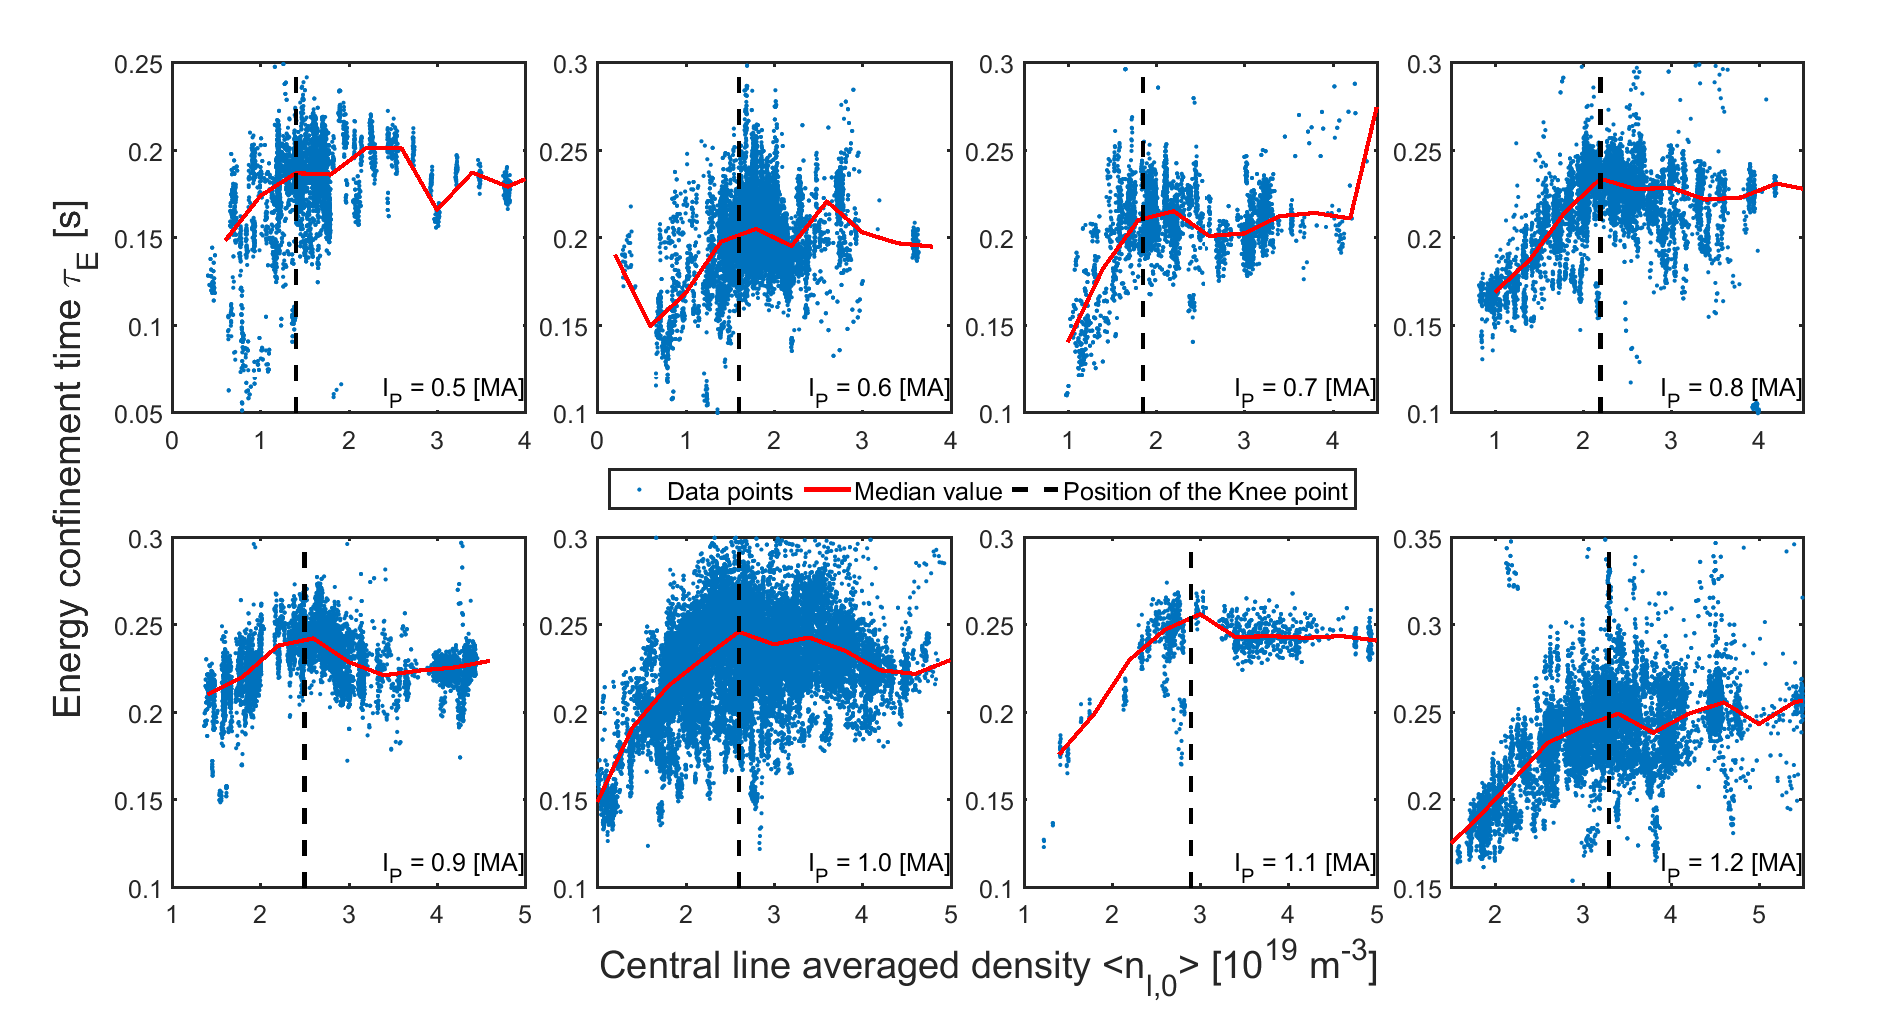
\includegraphics[scale=0.5]{fig_tau_vs_ne.eps}
\par\end{centering}
\caption{Evolution of the total energy confinement time with respect to the central line-averaged density at different plasma current.}
\label{fig:tau_vs_ne}
\end{figure}
%%%%%%%%%%%%%%%%%%%%


Figures \ref{fig:tau_vs_ne} and \ref{fig:nLOCSOC_Ip} describe the two steps to obtain the scaling of $n_\mathrm{LOC-SOC}$. First, at fixed $I_p$ in Ohmic plasmas, the total energy confinement time ($\tau_E$) increases with the central line-averaged density, passing a knee point at the approximate threshold density and then reaching saturation. Figure \ref{fig:tau_vs_ne} shows such an evolution of $\tau_E$ with line-averaged density ($n_l$) in the database for different $I_p$. To compensate for the scatter of the data, the median confinement time is calculated in small density ranges. The knee point of the median curve then provides the estimate of the LOC-SOC transition density threshold. Next, Figure \ref{fig:nLOCSOC_Ip} shows the evolution of the density threshold at different $I_p$ and the following scaling relation could be obtained by a linear fit:%
%%%%%%%%%%%%%%%%%%%%
\begin{equation}
  n_\mathrm{LOC-SOC}^\mathrm{TS} \approx 2.6 \times I_p,
\end{equation}
%%%%%%%%%%%%%%%%%%%%
\noindent with $n_\mathrm{LOC-SOC}$ in $10^{19}$ m$^{-3}$ and $I_p$ in MA. The LOC-SOC transition densities obtained from two dedicated density scans at $I_p= 0.5$ MA and 1.2 MA \cite{Arnichand_2014_NF} conform with the scaling law obtained from the database.

Finally, the central line-averaged density $n_{l,0}$ from interferometry measurements \cite{Gil_2009_FST} is used to determine the confinement regime for each reflectometer acquisition, assuming a $\pm$10\% uncertainty on the threshold given by the scaling law:%
%%%%%%%%%%%%%%%%%%%%
\begin{itemize}
  \item LOC: $n_{l,0} < 0.9 \times n_\mathrm{LOC-SOC}^\mathrm{TS}$;
  \item SOC: $n_{l,0} > 1.1 \times n_\mathrm{LOC-SOC}^\mathrm{TS}$.
\end{itemize}
%%%%%%%%%%%%%%%%%%%%
\noindent In the remainder, we refer to the intermediate region around the density threshold as the \emph{LOC-SOC transition regime}.


%%%%%%%%%%%%%%%%%%%%
\begin{figure}[h]
\begin{centering}
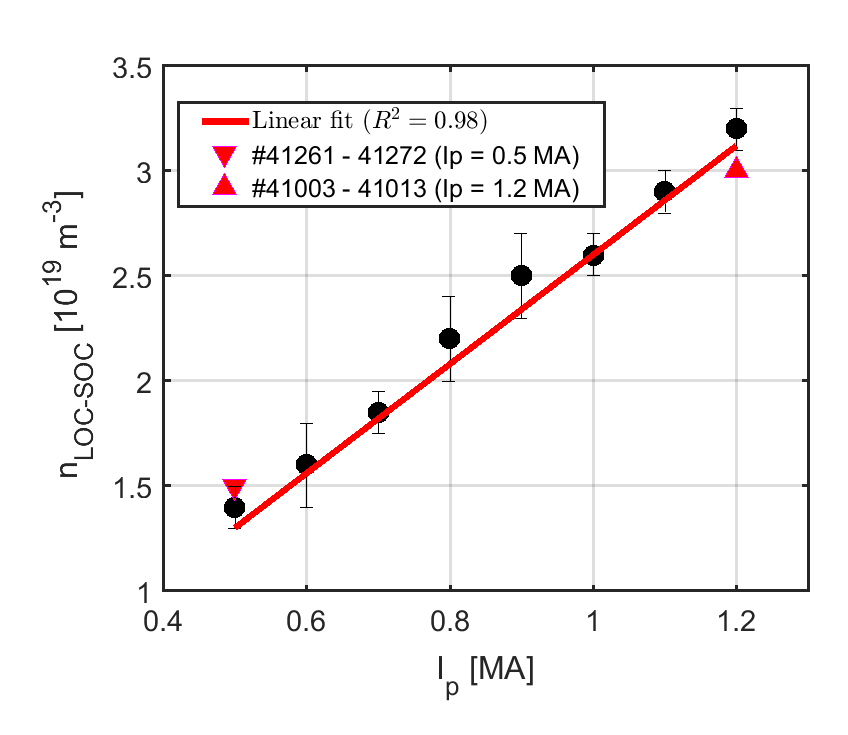
\includegraphics[scale=0.65]{fig_nLOCSOC_Ip.eps}
\par\end{centering}
\caption{Empirical scaling law of the LOC-SOC transition density threshold ($n_\mathrm{LOC-SOC}$) in terms of plasma current ($I_p$).}
\label{fig:nLOCSOC_Ip}
\end{figure}
%%%%%%%%%%%%%%%%%%%%


\subsection{Radial profiles of $E_\mathrm{BB}$}

Having discriminated between the LOC and SOC regimes, the radial profiles of $E_\mathrm{BB}$ can be studied separately in both regimes. Figure \ref{fig:ELS} shows the $E_\mathrm{BB}$ profiles at different range of $q_{\psi}$. Compared to the Ohmic cases in figure \ref{fig:EBBOhmic}, the general evolution of $E_\mathrm{BB}$ across the radial extent of the plasma, as well as the $E_\mathrm{BB}$ basin in the central region, are recovered in both LOC and SOC regimes for all $q_{\psi}$ ranges. The analysis also recovers the link between the basin (width, location) and the $q = 1$ surface. Far outside the $q = 1$ surface at the LFS, $E_\mathrm{BB}$ approaches 1 in both regimes, i.e. with most of the energy in the BB component, whereas at the HFS $E_\mathrm{BB}$ remains at a moderate level. In fact, the general trends become more clear after separating the Ohmic plasmas into the two confinement regimes, as the data in a fixed radial position are less scattered, especially for the LOC regime.

Furthermore, remarkable differences occur for the two regimes, i.e, the magnitude of $E_\mathrm{BB}$. At the same range of $q_{\psi}$, $E_\mathrm{BB}$ in SOC is systematically higher than in LOC, which is valid for all $q_{\psi}$. Note that since the cutoff positions depend on density, the LFS for the LOC regime is less accessible at higher $q_{\psi}$ ($5 < q_{\psi} < 6$ and $6 < q_{\psi} < 10$), whereas for the SOC regime only the HFS at the lowest $q_{\psi}$ range is less accessible.

To achieve a better comparison of $E_\mathrm{BB}$ between the two regimes, the median values for each $q_{\psi}$ range were calculated by the same method as in the Ohmic case (figure \ref{fig:EBBOhmic}). Figure \ref{fig:ELS_med} shows the radial profiles of the median values for the two regimes, while the original data points have been hidden in view of the strong overlap between the LOC and SOC regimes. The systematically higher $E_\mathrm{BB}$ in the SOC regime than in the LOC regime, throughout the plasma cross-section for all $q_{\psi}$, is clearly confirmed. Specifically, for the LOC regime inside the $q = 1$ surface, $E_\mathrm{BB}$ is very low, especially at low $q_{\psi}$. This means that for the LOC regime in the very core region ($\rho \sim 0$) only a minor part of the energy is in the BB component, or equivalently, most of the energy of the frequency spectra is in the LF component. In contrast, in the SOC regime $E_\mathrm{BB}$ can still reach levels of 20\% at $\rho \sim 0$.


%%%%%%%%%%%%%%%%%%%%
\begin{figure}[h]
\begin{centering}
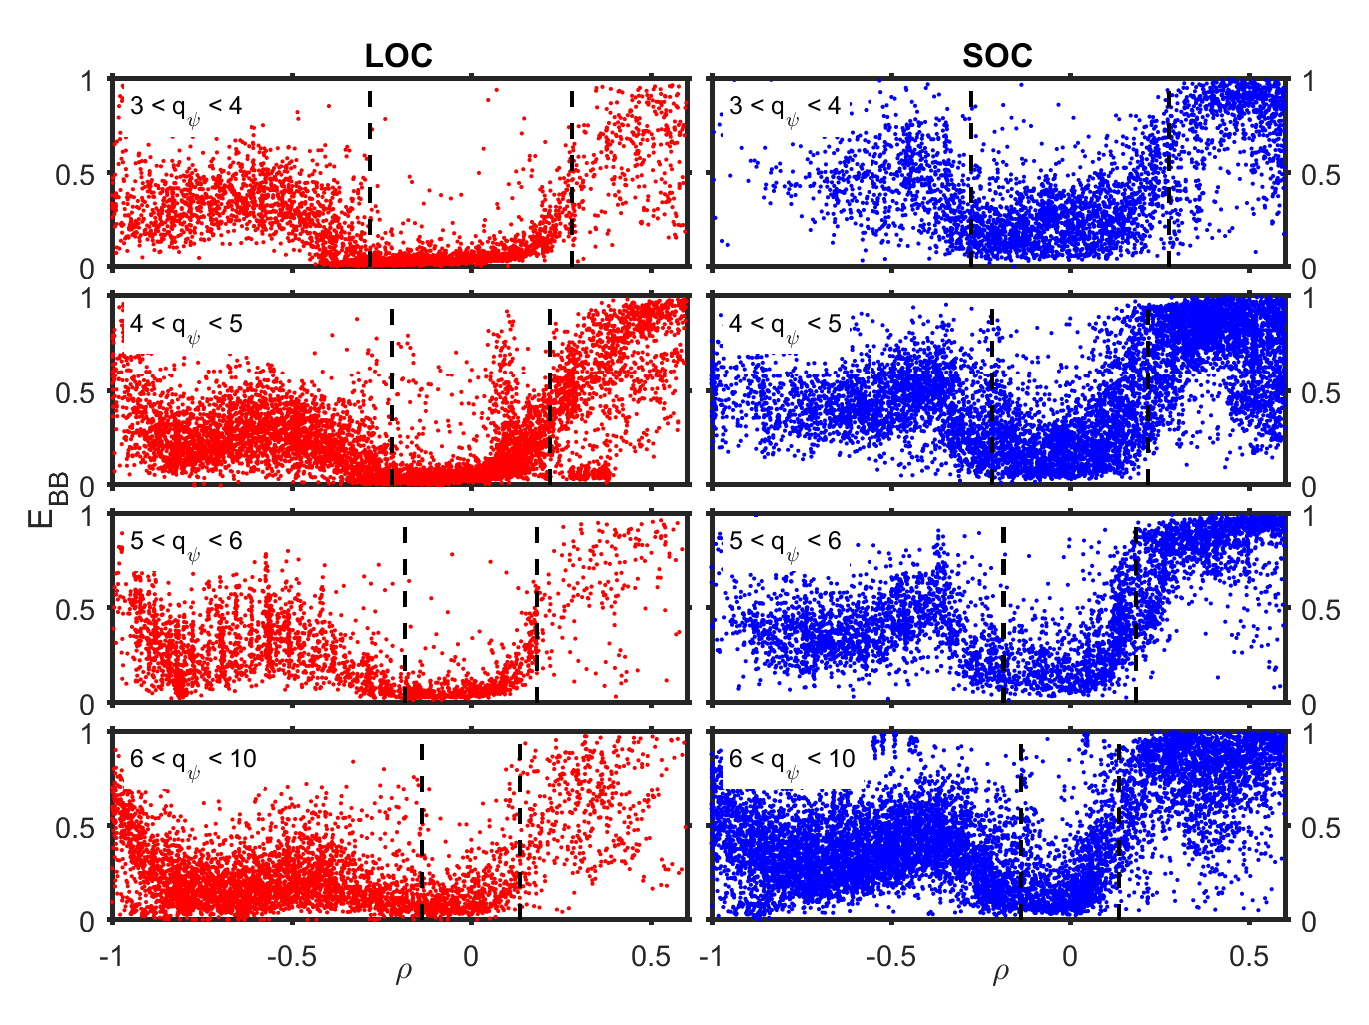
\includegraphics[scale=0.65]{fig_EBB_LOCSOC.eps}
\par\end{centering}
\caption{Radial profiles of $E_\mathrm{BB}$ at different $q_{\psi}$ in the linear Ohmic confinement (LOC) and the saturated Ohmic confinement (SOC). The approximate $q = 1$ surface is shown by the black dashed line for each condition.}
\label{fig:ELS}
\end{figure}
%%%%%%%%%%%%%%%%%%%%


For a more quantitative study, the central $E_\mathrm{BB}$ basin is defined as the corresponding radial range where the median values are below 0.2. Then, $E_\mathrm{BB}$ inside the basin for both LOC and SOC is plotted as a function of $q_{\psi}$ in figure \ref{fig:EBBtrendLS}. Remarkable is the higher $E_\mathrm{BB}$ inside the basin in the SOC regime, compared to the LOC regime, for all $q_{\psi}$. The difference between the two regimes disappears at highest $q_{\psi}$ due to the different trends of $E_\mathrm{BB}$ with respect to $q_{\psi}$. Specifically, with increasing $q_{psi}$, $E_\mathrm{BB}^\mathrm{LOC}$ increases rapidly before saturation around $E_\mathrm{BB} \approx 0.2$ at high $q_{\psi}$, whereas $E_\mathrm{BB}^\mathrm{SOC}$ decreases slowly to $0.2$ at high $q_{\psi}$. %The difference between the LOC and SOC regimes might be related to different turbulence characteristics in the two confinement regimes. This is to be studied in more detail, as some parameters have not been considered in this preliminary analysis, e.g. the density or collisionality.


%%%%%%%%%%%%%%%%%%%%
\begin{figure}[h]
\begin{centering}
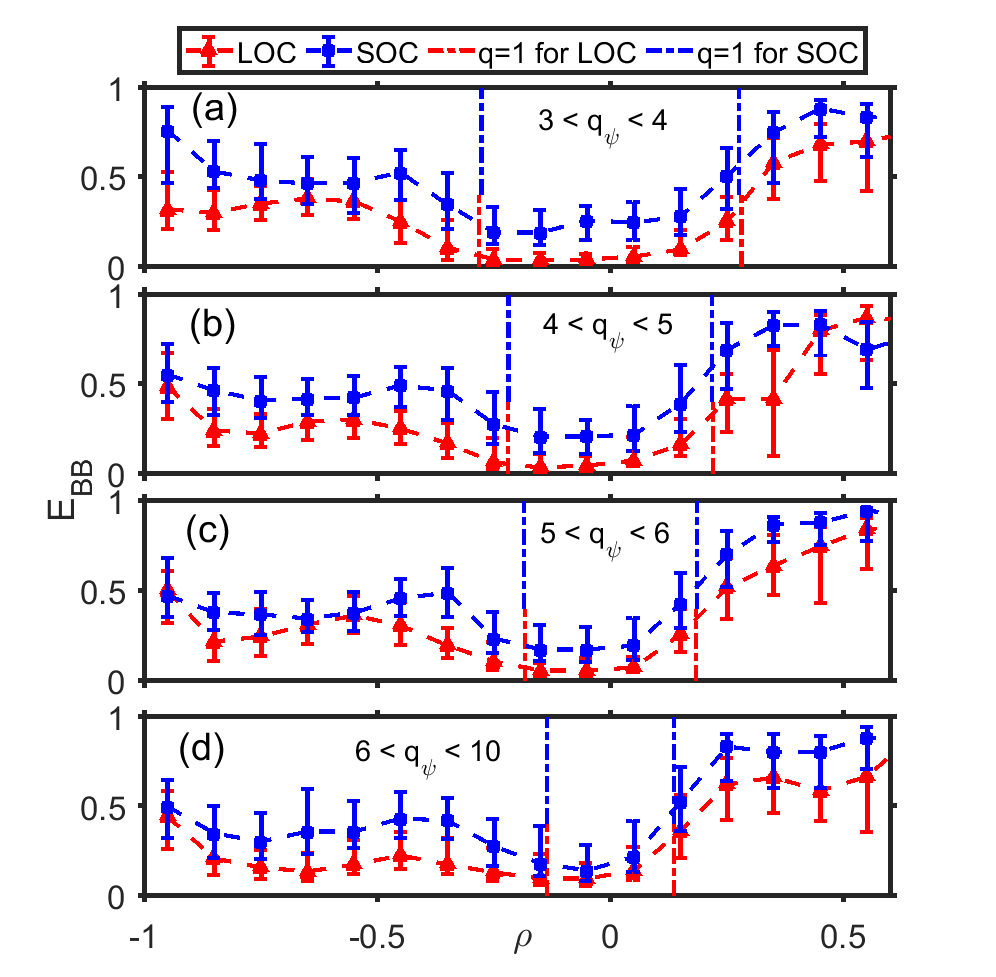
\includegraphics[scale=0.6]{fig_EBB_LOCSOC_med.eps}
\par\end{centering}
\caption{Median radial profiles of $E_\mathrm{BB}$ for different $q_{\psi}$ in the LOC and SOC regimes. The approximations of the $q = 1$ positions were obtained separately for both regimes by the same method as in figure \ref{fig:EBBOhmic}.}
\label{fig:ELS_med}
\end{figure}
%%%%%%%%%%%%%%%%%%%%


%%%%%%%%%%%%%%%%%%%%
\begin{figure}[!h]
\begin{centering}
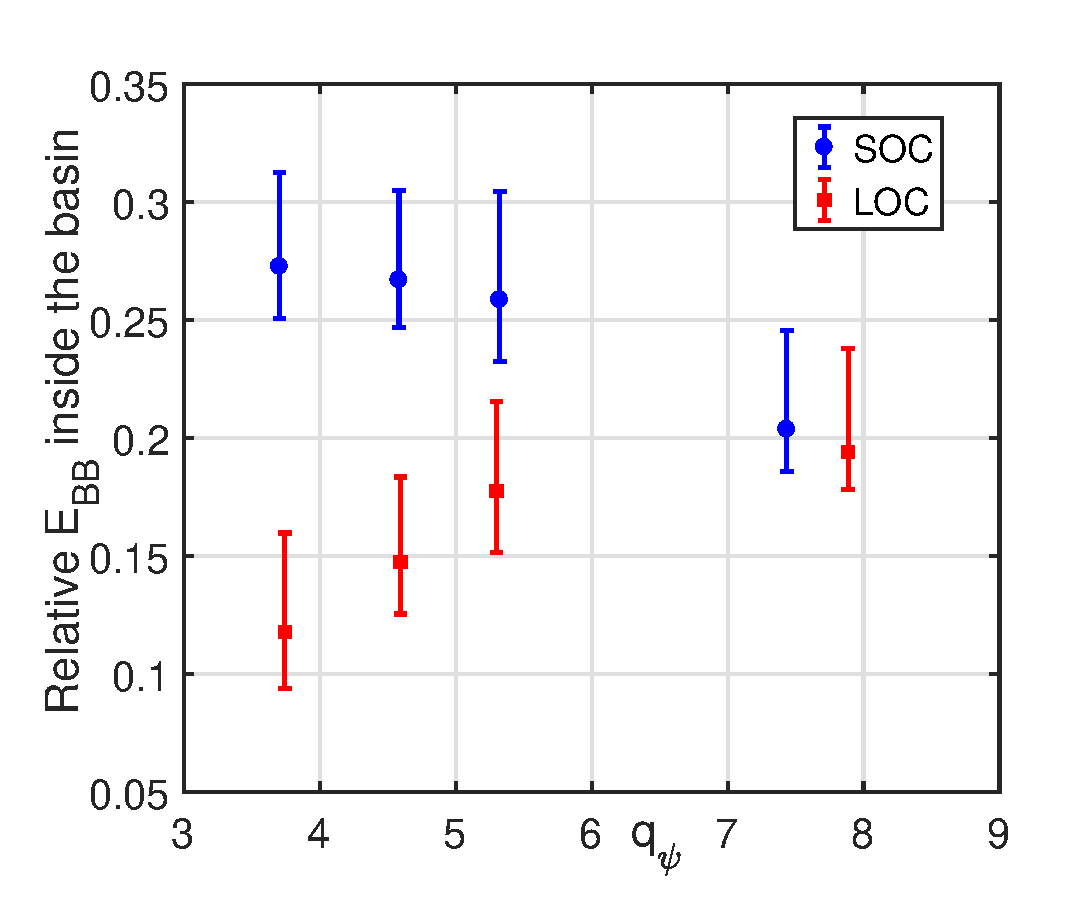
\includegraphics[scale=0.45]{fig_Trend_LOCSOC.eps}
\par\end{centering}
\caption{Evolution of $E_\mathrm{BB}$ inside the $E_\mathrm{BB}$ basin with respect to $q_{\psi}$ in the LOC and SOC regimes.}
\label{fig:EBBtrendLS}
\end{figure}
%%%%%%%%%%%%%%%%%%%%


\section{Broadband contribution in terms of injected power} \label{sec:radial_profile_ICRH_LH}

Having investigated Ohmic plasmas, we now turn to the case with auxiliary heating. In Tore Supra, ICRH and LH are the two most commonly applied methods for auxiliary heating or current drive. Note that most of the Tore Supra discharges with LH were devoted to current drive, allowing the appearance of fast electrons and thus varying ratios of trapped electrons. For clarity, we focus on plasmas that are either pure ICRH or LH plasmas.

Radial profiles of the BB contribution at different ranges of the edge safety factor and heating power are shown in Figures \ref{fig:EBB_ICRH} (ICRH) and \ref{fig:EBB_LH} (LH). The $E_\mathrm{BB}$ profiles in Ohmic plasmas with the same range of $q_{\psi}$ are shown for comparison.


\subsection{Radial profiles of $E_\mathrm{BB}$ with ICRH} \label{sec:EBB_ICRH}

From figure \ref{fig:EBB_ICRH}, it is clear that $E_\mathrm{BB}$ is generally considerably higher with ICRH than in Ohmic plasmas, approaching the Ohmic $E_\mathrm{BB}$ only far outside the $q = 1$ surface. The global increase of $E_\mathrm{BB}$ should be related to a higher turbulence level with ICRH due to a larger temperature gradient. Specifically, towards the LFS, almost all of the energy is in the broadband component. At the HFS and inside the central basin, $E_\mathrm{BB}$ increases with increasing heating power. At fixed heating power, a slight rise of $E_\mathrm{BB}$ is also observed with increasing $q_{\psi}$. This rise corresponds to an increase of the fluctuation level due to the degradation of the confinement with increasing $q_{\psi}$ (i.e. decreasing $I_p$). This rise has not been observed for the Ohmic cases, because $I_p$ is used as a heating source in Ohmic plasmas and thus the situation is more complicated. Note that at the HFS near the edge, $E_\mathrm{BB}$ is clearly lower than in the core region. The higher $E_\mathrm{BB}$ in the core might be caused by fast particles, as the ICRH power deposition occurs mainly in the core at Tore Supra. Specifically, at the lowest ICRH heating powers (0.5 MW $< P_\mathrm{ICRH} <$ 1.5 MW), there is a clear $E_\mathrm{BB}$ basin in the core, but it becomes shallower with increasing $P_\mathrm{ICRH}$, and almost disappears when $P_\mathrm{ICRH} > $ 2.5 MW. This trend is observed for all $q_{\psi}$ ranges.


%%%%%%%%%%%%%%%%%%%%
\begin{figure}[h]
\begin{centering}
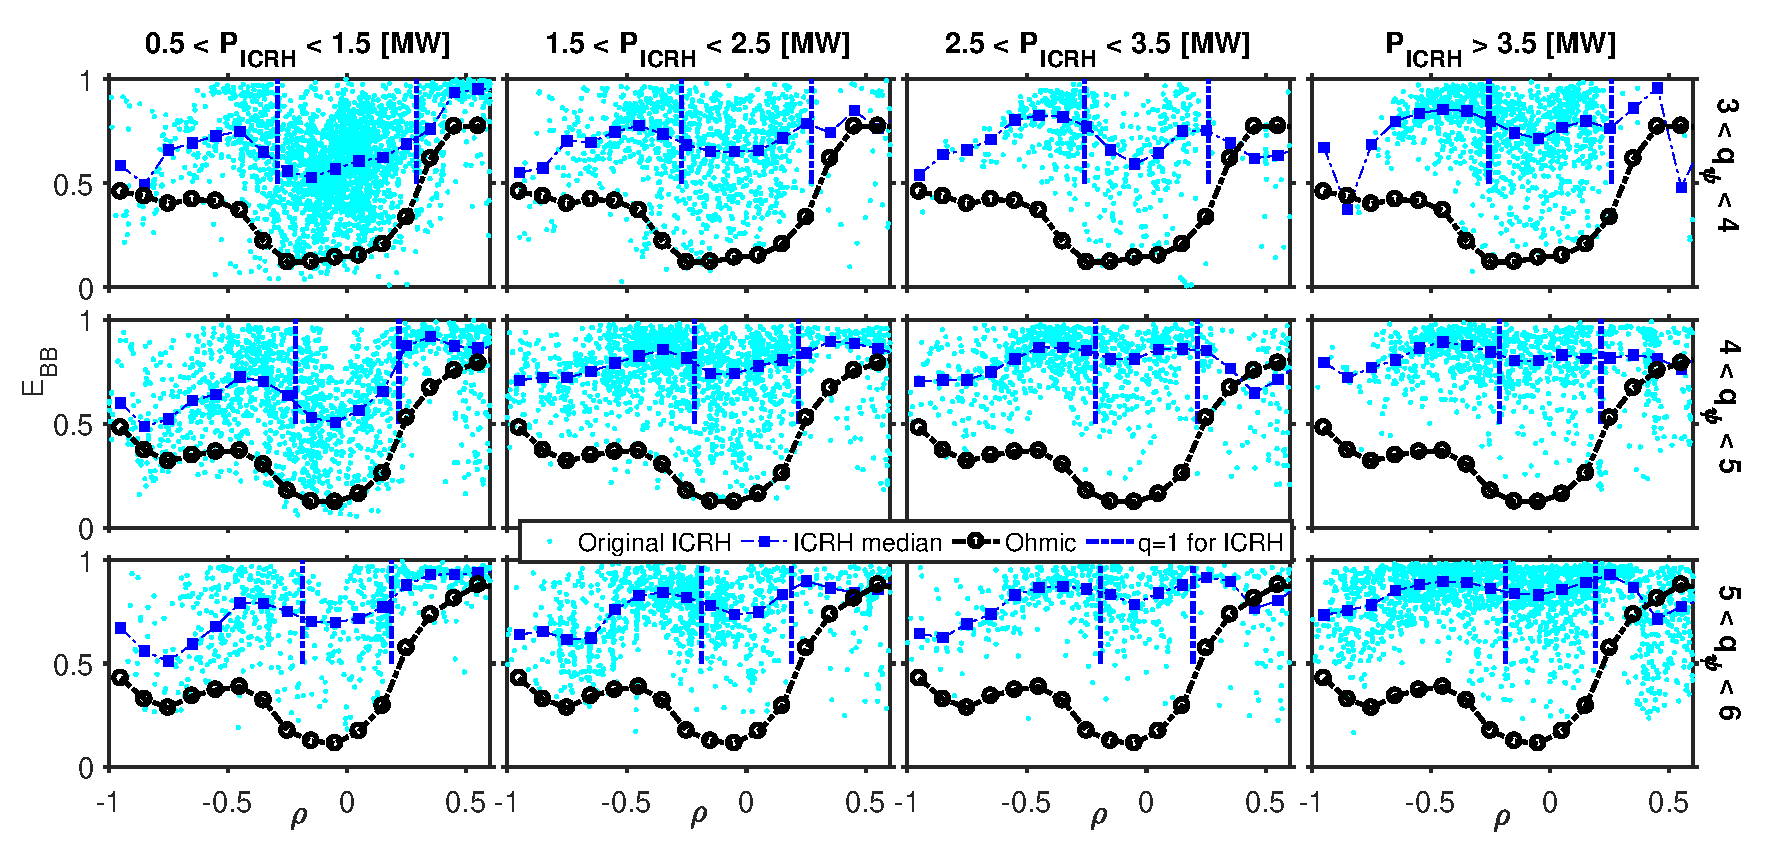
\includegraphics[scale=0.535]{fig_EBB_ICRH.eps}
\par\end{centering}
\caption{Radial profiles of $E_\mathrm{BB}$ in pure ICRH plasmas (blue) with various ranges of heating power and $q_{\psi}$. The $q = 1$ surface for the ICRH plasmas is indicated by the vertical dashed lines in each panel. $E_\mathrm{BB}$ profiles in Ohmic plasmas (black) are shown for comparison.}
\label{fig:EBB_ICRH}
\end{figure}
%%%%%%%%%%%%%%%%%%%%


\subsection{Radial profiles of $E_\mathrm{BB}$ with LH} \label{sec:EBB_LH}

For the LH plasmas shown in figure \ref{fig:EBB_LH}, the $E_\mathrm{BB}$ basin linked to the $q = 1$ surface remains visible even at very high power ($P_{LH}>3$ MW). $E_\mathrm{BB}$ slightly increases along part of the radius with increasing $P_{LH}$. At fixed heating power, $E_\mathrm{BB}$ inside the $q = 1$ surface sightly increases with increasing $q_{\psi}$. The different behavior of the $E_\mathrm{BB}$ basin in LH and ICRH plasmas may be linked to differences in the temperature profile inside the $q = 1$ surface for ICRH vs. LH.

A large scatter of $E_\mathrm{BB}$ at fixed radial position can be noted for both ICRH and LH plasmas, although the scatter is weaker inside the $q = 1$ surface for LH plasmas. Since the $q = 1$ surface is linked with the sawtooth instability, the evolution of $E_\mathrm{BB}$ during the sawtooth period has been investigated. However, no clear change of the $E_\mathrm{BB}$ intensity has been observed, except at the time of the sawtooth crash.




%%%%%%%%%%%%%%%%%%%%
\begin{figure}[h]
\begin{centering}
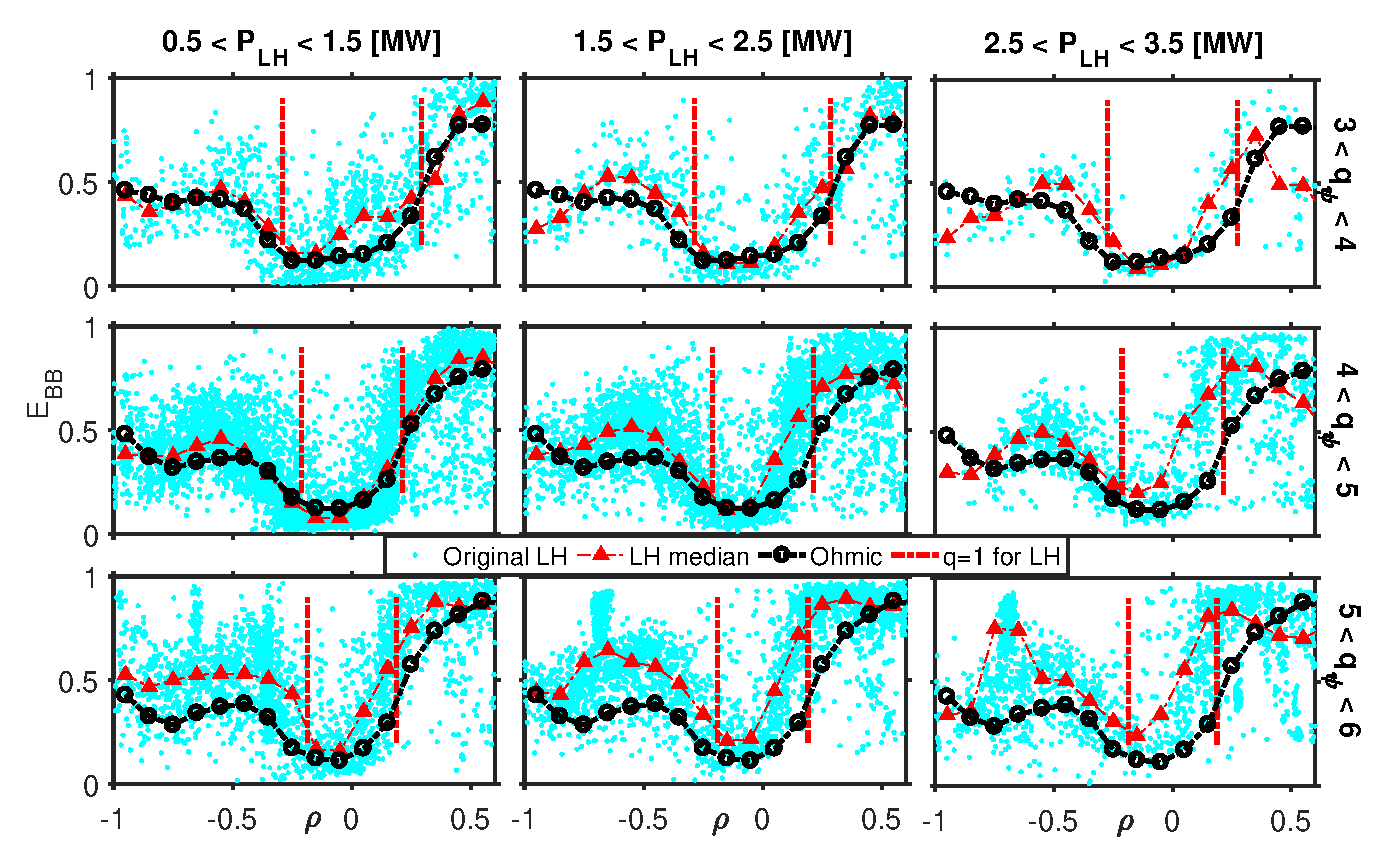
\includegraphics[scale=0.5]{fig_EBB_LH.eps}
\par\end{centering}
\caption{Same as in figure \ref{fig:EBB_ICRH} in LH plasmas (the highest power range is not reached).}
\label{fig:EBB_LH}
\end{figure}
%%%%%%%%%%%%%%%%%%%%


Most noticeably, in the central region and at the HFS, there are significant differences between the $E_\mathrm{BB}$ profiles in plasmas with ICRH vs. LH. In particular, in LH-heated plasmas, $E_\mathrm{BB}$ is limited, below $< 0.5$, at the HFS and central region, especially in the latter ($0.1 < E_\mathrm{BB} < 0.2$). In contrast, with ICRH, $E_\mathrm{BB}$ goes well above 0.5 for all radii, reaching levels of 0.7--0.8 in the central region and at the HFS, and even higher at the LFS.


\section{$E_\mathrm{BB}$ in terms of fluctuation level} \label{sec:EBB2dn}

The radial profiles of $E_\mathrm{BB}$ in Ohmic plasmas identified in figure \ref{fig:EBBOhmic} from the database, can be compared to a previous study of the density fluctuation level ($\delta n/n$) in a dedicated discharge \#35035 from \cite{Sabot_2006_PPCF}, as shown in figure \ref{fig:fluc_level_ohmic} (a). Comparing the radial profiles of $E_\mathrm{BB}$ and $\delta n/n$, the basin structure inside the $q = 1$ surface and the strong asymmetry between the HFS and LFS are similar. Even the slow increase of $\delta n/n$ from the edge towards the center at the HFS in figure \ref{fig:fluc_level_ohmic} (a) has also been recovered systematically in figure \ref{fig:EBBOhmic}. There is a difference between the radial profiles of $E_\mathrm{BB}$ and $\delta n/n$ at the LFS, where $E_\mathrm{BB}$ saturates, whereas $\delta n/n$ increases monotonically. In this section, we try to establish a link between $E_\mathrm{BB}$ and $\delta n/n$.


\subsection{Confirmation of the general trends of $E_\mathrm{BB}$}

Note that when constructing the radial profiles of $E_\mathrm{BB}$, the spectra were calculated originally from the complex signal and the normalized $E_\mathrm{BB}$ has been used so far. These factors might cause a distortion of the radial profiles of $E_\mathrm{BB}$ and are considered in the following to confirm the general trends.


\subsubsection{Different acquisition methods}

%%%%%%%%%%%%%%%%%%%%
\begin{figure}[h]
\begin{centering}
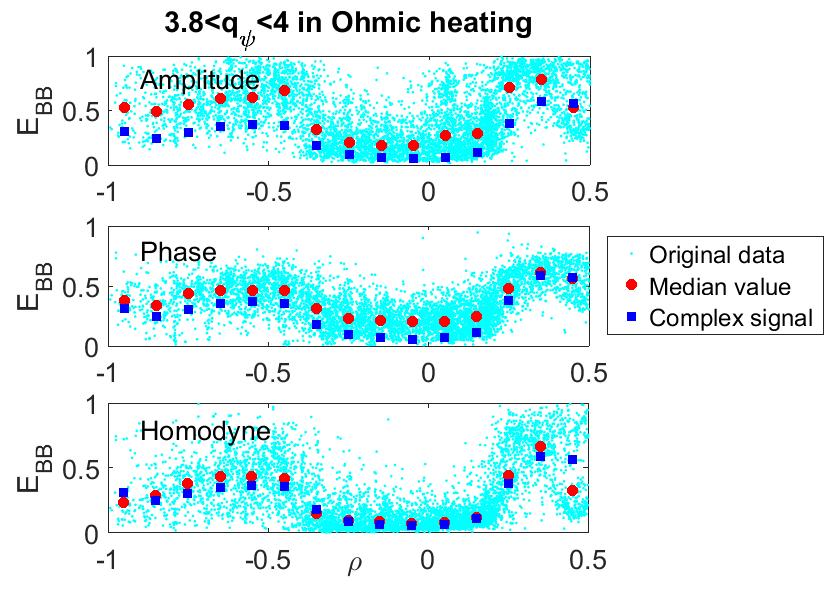
\includegraphics[scale=0.5]{fig_EBB_Amp_Phase_Homo_OH.jpg}
\par\end{centering}
\caption{Radial profiles of $E_\mathrm{BB}$ by amplitude, phase and homodyne signals compared with the complex signals used in this study.}
\label{fig:EBB_Amp_Phase_Homo_OH}
\end{figure}
%%%%%%%%%%%%%%%%%%%%

First, to confirm that the general trends of $E_\mathrm{BB}$ observed are independent of the acquisition technique (heterodyne vs. homodyne), we apply the parametrization method to the amplitude (A), the phase ($\phi$) and the homodyne signal (Asin($\phi$) or Acos($\phi$)) \cite{Blanco_2013_PPCF,Fernandez-Marina_2014_NF} of the complex signal obtained in this study. Without loss of generality, part of the full database ($3.8 < q_{\psi} < 4$) has been used in the comparison to reduce the computational requirements of the test. Figure \ref{fig:EBB_Amp_Phase_Homo_OH} shows the radial profiles of $E_\mathrm{BB}$ using the three different acquisition techniques, along with the median values for each case. The results using the complex signals are also depicted for comparison. Although some differences among the various signals exist, the general trends of the radial profiles are consistent. Specifically, $E_\mathrm{BB}$ obtained from the amplitude or phase signals is systematically higher than the complex signal, and the result from the homodyne signal is consistent with the complex signal. The discrepancy near $\rho = 0.5$ at the LFS is expected since the data points are more scattered in this region and are thus less reliable.


\subsubsection{Radial profiles of the unnormalized $E_\mathrm{BB}$}

Next, we consider the unnormalized $E_\mathrm{BB}$, which is the original energy fraction of the BB component without normalizing to the total power of each spectrum. The unnormalized $E_\mathrm{BB}$ is referred to as $E_\mathrm{BB}^\mathrm{unnorm}$ for clarity. Due to the normalization, $E_\mathrm{BB}$ is also affected by the other components of the frequency spectra, especially the LF component, which could affect the radial profiles of the BB contribution. Moreover, the different behavior of $E_\mathrm{BB}$ and $\delta n/n$ at the LFS suggests that $E_\mathrm{BB}^\mathrm{unnorm}$ might also be affected in this region. However, the large variation of the original spectrum power even at a fixed frequency (up to 60 dB) would blur the any radial trends, hence our preference for the normalized $E_\mathrm{BB}$. Taking this into account, we limit the reflected power range variation (a band of 9 dB around the maximum of the reflected spectra energy) and select a frequency range (115--140 GHz) in which the reflectometer detection efficiency is the most stable (limited variation of the multiplier output and mixer conversion loss).

Figure \ref{fig:EBB_unnorm_OH} (a) shows the radial profile of $E_\mathrm{BB}^\mathrm{un-norm}$ at $3 < q_{\psi} < 4$ at selected spectral powers and frequencies. Inside the $q = 1$ surface, $E_\mathrm{BB}^\mathrm{un-norm}$ remains small with low dispersion, whereas outside the $q = 1$ surface, $E_\mathrm{BB}^\mathrm{un-norm}$ is much higher with strong dispersion at both the HFS and LFS. Moreover, $E_\mathrm{BB}^\mathrm{un-norm}$ at the LFS is systematically higher than at the HFS. Due to the large difference of $E_\mathrm{BB}^\mathrm{un-norm}$ between the core and edge region, the radial profile is also shown on the logarithmic scale (Figure \ref{fig:EBB_unnorm_OH} (b)). From the V-shaped trend through the cross-section, we deduce that $E_\mathrm{BB}^\mathrm{un-norm}$ decreases almost exponentially from the edge to the core region. The observations from $E_\mathrm{BB}^\mathrm{un-norm}$ again confirm the general trends from figure \ref{fig:EBBOhmic}.

Moreover, since $E_\mathrm{BB}^\mathrm{un-norm}$ should be more directly linked to the measurements of phase fluctuations ($\delta\phi$) by reflectometers, as opposed to density fluctuations ($\delta n/n$), the factor connecting $\delta n/n$ to $\delta\phi$ should be considered. From section \ref{sec:dphi2dn}, $\delta\phi$ is related to $\delta n/n$ as \cite{Shelukhin_2006_PPR}:%
%%%%%%%%%%%%%%%%%%%%
\begin{equation}
  \delta\phi \propto \sqrt{\frac{L_{\epsilon} \Delta_r^{cor}}{\lambda_0}}\frac{\delta n}{n},
\end{equation}
%%%%%%%%%%%%%%%%%%%%
\noindent where $L_{\epsilon}=(\partial\epsilon/\partial r)^{-1}$ is the scale length of the plasma permittivity $\epsilon$ at the cutoff position, $\lambda_0$ the wavelength of the probing wave and $\Delta_r^{cor} \approx 1/k_\mathrm{eff}$ the turbulence radial correlation length. Therefore, in order to recover the radial profiles of $\delta n/n$, a correction factor $\sqrt{\frac{L_{\epsilon} \Delta_r^{cor}}{\lambda_0}}$ should be taken into account. The turbulence correlation length $\Delta_r^{cor}$ is not available for the whole database and is assumed to be constant ($\sim 1$ cm) across the radial cross-section. Figure \ref{fig:EBB_unnorm_OH} (c) and (d) show the radial profiles of $E_\mathrm{BB}^\mathrm{un-norm}$ considering the correction factor in the linear and logarithmic scale, respectively, exhibiting similar trends. The dispersion of the data is significantly reduced, indicating a better recovery of the trends after adding the correction factor.


%%%%%%%%%%%%%%%%%%%%
\begin{figure}[h]
\begin{centering}
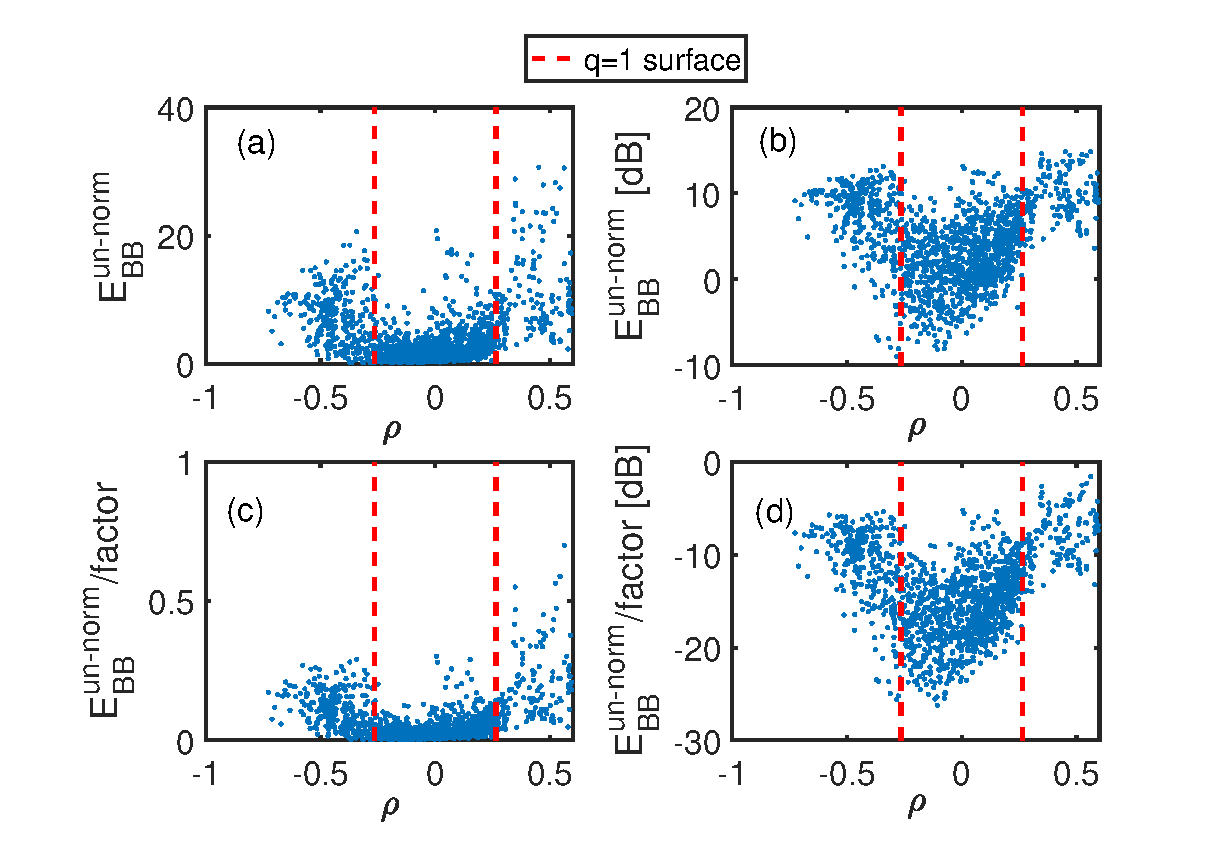
\includegraphics[scale=0.8]{fig_EBB_unnorm_vs_r_q34.eps}
\par\end{centering}
\caption{Radial profiles of the unnormalized $E_\mathrm{BB}$ ($E_\mathrm{BB}^\mathrm{unnorm}$) in the (a) linear and (b) logarithmic scale. Radial profiles of $E_\mathrm{BB}^\mathrm{unnorm}$ considering the correction factor in the (c) linear and (d) logarithmic scale. The edge safety factor is in the range $3 < q_{\psi} < 4$. The approximate $q = 1$ positions are indicated by the red vertical dashed line.}
\label{fig:EBB_unnorm_OH}
\end{figure}
%%%%%%%%%%%%%%%%%%%%


\subsection{Radial profiles of the corrected $E_\mathrm{BB}$}

Although $E_\mathrm{BB}^\mathrm{un-norm}$ may be more directly linked to the turbulence level than $E_\mathrm{BB}$, the application of $E_\mathrm{BB}^\mathrm{un-norm}$ to a large database requires strong constraints on power and frequency. Therefore, to conduct a systematic study without these limits, we focus on $E_\mathrm{BB}$, which can be calculated for the entire database without limitations. The analysis of $E_\mathrm{BB}^\mathrm{unnorm}$ could be a complementary parameter when investigating dedicated discharges in a deeper study. On the other hand, the correction factor $\sqrt{\frac{L_{\epsilon} \Delta_r^{cor}}{\lambda_0}}$ might help to strengthen the general trends (as shown in figure \ref{fig:EBB_unnorm_OH}).

First, we consider the correction factor in the study of the radial profiles of $E_\mathrm{BB}$ in Ohmic plasmas, as shown in figure \ref{fig:EBB_correct_OH}. As expected, the general trends of the corrected $E_\mathrm{BB}$ ($E_\mathrm{BB}$/factor) are consistent with the results from $E_\mathrm{BB}$ with reduced data dispersion at fixed radial positions. The only difference lies at the LFS near the plasma edge, where the corrected $E_\mathrm{BB}$ increases monotonically from the core towards the edge. This is consistent with the radial profiles of $\delta n/n$.


%%%%%%%%%%%%%%%%%%%%
\begin{figure}[h]
\begin{centering}
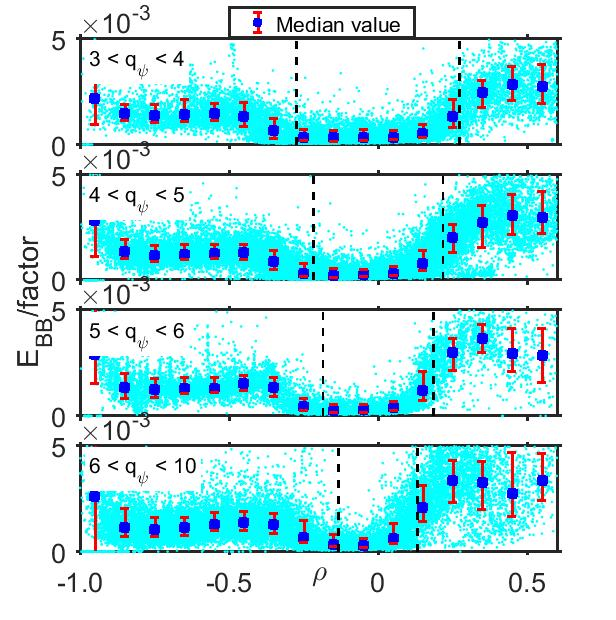
\includegraphics[scale=0.5]{fig_EBB_correct_OH.jpg}
\par\end{centering}
\caption{Same as figure \ref{fig:EBBOhmic}, but considering the correction factor $\sqrt{\frac{L_{\epsilon} \Delta_r^{cor}}{\lambda_0}}$.}
\label{fig:EBB_correct_OH}
\end{figure}
%%%%%%%%%%%%%%%%%%%%


Furthermore, we extend the analysis to L-mode plasmas with auxiliary power. In order to systematically compare the results of turbulence level (figure \ref{fig:fluc_level_heating}) from previous studies \cite{Guirlet_2010_NF}, similar ranges of heating power of ICRH and LH have been selected. Figure \ref{fig:EBBc_ICRH_LH} shows the radial profiles of the corrected $E_\mathrm{BB}$ in ICRH or LH plasmas. The radial profile in Ohmic plasmas at corresponding $q_{\psi}$ is also shown for comparison. From figure \ref{fig:EBBc_ICRH_LH}, the radial profiles of the turbulence level from figure \ref{fig:fluc_level_heating} has been systematically recovered for a much larger range of plasma conditions. Specifically, the dedicated LH-dominated discharge of figure \ref{fig:fluc_level_heating} has a fraction (25\%) of ICRH. However, in our database study, for the selected range of parameters ($q_{\psi}$ and power), there are only a few discharges with similar LH and ICRH power. It was thus preferred to show the pure LH cases. This explains the small difference between shot \#34931 of figure \ref{fig:fluc_level_heating} and the LH cases in figure \ref{fig:EBBc_ICRH_LH}. Moreover, the results shown in figure \ref{fig:EBBc_ICRH_LH} are only an example of the full parameter range, as shown by figures \ref{fig:EBB_ICRH} and \ref{fig:EBB_LH} (and also figure \ref{fig:EBBOhmic}).


The remarkable difference between the BB contribution shown in figures \ref{fig:EBB_ICRH}, \ref{fig:EBB_LH} and \ref{fig:EBBc_ICRH_LH} for ICRH and LH plasmas with similar heating power lead us to investigate further. Figure \ref{fig:EBB_diff_ICRH_LH} (a) shows the $E_\mathrm{BB}$ in the core for ICRH and LH plasmas at different heating power. $E_\mathrm{BB}$ in the core increases almost linearly with heating power for both ICRH and LH plasmas and $E_\mathrm{BB}$ with ICRH is systematically higher than with LH for all heating powers. The difference of $E_\mathrm{BB}$ between ICRH and LH is almost independent of the heating power. To understand the origins of the discrepancy, we have investigated the corresponding energy confinement time ($\tau_{E}$) at different power for ICRH and LH plasmas, as shown in figure \ref{fig:EBB_diff_ICRH_LH} (b). Here, a median value of the confinement time in the range of heating power has been used. The differences of $\tau_{E}$ among ICRH and LH plasmas are much smaller than the differences of $E_\mathrm{BB}$. Importantly, this suggests that the huge difference of $E_\mathrm{BB}$ between ICRH and LH plasmas cannot be explained by a degradation of confinement, and therefore some other mechanism must be at work.


%%%%%%%%%%%%%%%%%%%%
\begin{figure}[h]
\begin{centering}
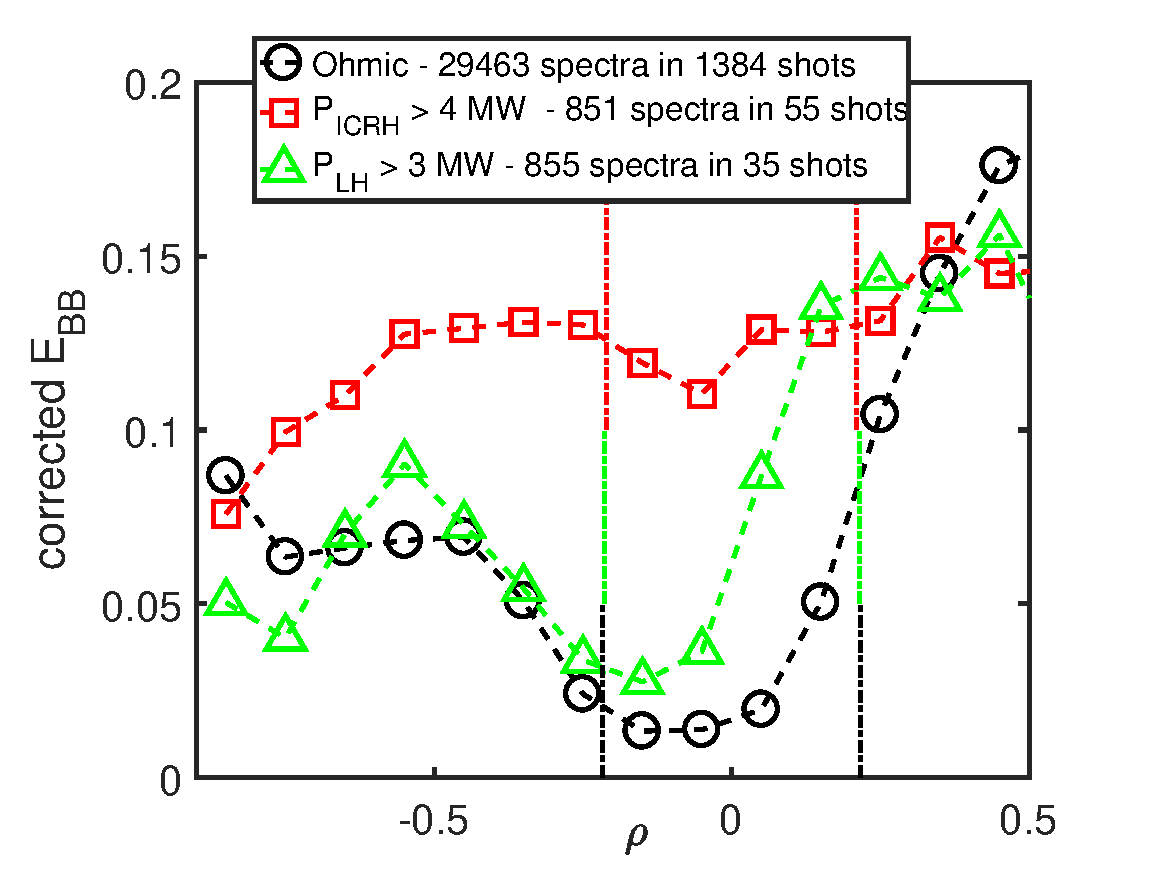
\includegraphics[scale=0.6]{fig_EBBc_ICRH_LH.eps}
\par\end{centering}
\caption{Radial profiles of $E_\mathrm{BB}$ in Ohmic, ICRH and LH plasmas under the condition $4 < q_{\psi} < 5$. The $q = 1$ positions are indicated by the vertical dashed lines with the corresponding color.}
\label{fig:EBBc_ICRH_LH}
\end{figure}
%%%%%%%%%%%%%%%%%%%%


%%%%%%%%%%%%%%%%%%%%
\begin{figure}[h]
\begin{centering}
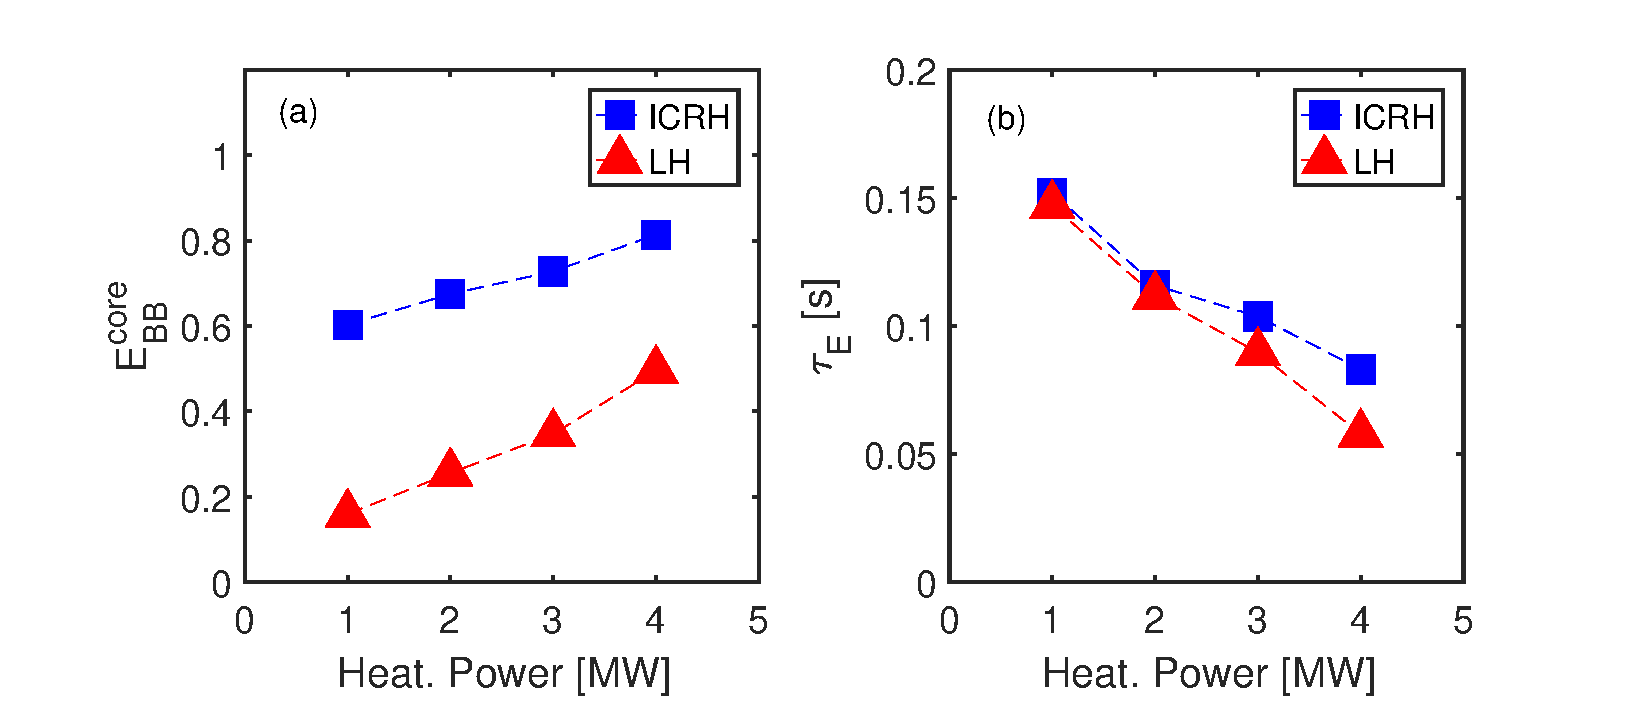
\includegraphics[scale=0.6]{fig_EBB_diff_ICRH_LH.eps}
\par\end{centering}
\caption{(a) $E_\mathrm{BB}$ inside the $q = 1$ surface and (b) the energy confinement time at different heating power for ICRH and LH plasmas for a large range of edge safety factor ($q_{\psi}$)).}
\label{fig:EBB_diff_ICRH_LH}
\end{figure}
%%%%%%%%%%%%%%%%%%%%


\section{Summary and discussion} \label{summary_discussion}

Radial profiles of the BB contribution in frequency spectra have been systematically studied for both Ohmic and L-mode plasmas with ICRH and LH heating. The general observed trends are summarized in the following:
%%%%%%%%%%%%%%%%%%%%
\begin{itemize}

  \item In Ohmic plasmas, a drastic reduction of the BB contribution, called the $E_\mathrm{BB}$ basin, is observed inside the core region. The position and width of the reduction are correlated with the $q = 1$ surface. A strong asymmetry of the BB contribution exists at the HFS and LFS.

  \item In the LOC and SOC regimes, the trends observed in Ohmic plasmas are strengthened. Moreover, the BB contribution in the SOC regime is systematically higher than in the LOC regime.

  \item For the auxiliary heating case, the $E_\mathrm{BB}$ basin is recovered in the pure LH plasmas, whereas for the pure ICRH plasmas, the basin disappears even at low heating power. In addition, with increasing heating power or edge safety factor, the BB contribution increases for both ICRH and LH plasmas.

\end{itemize}
%%%%%%%%%%%%%%%%%%%%

The radial profiles of $E_\mathrm{BB}$ systematically recover the profiles of the turbulence level obtained in earlier dedicated studies. Hence, we have been able to systematically reconstruct the turbulence level in an automated way across a large data set. However, the turbulence correlation length is not available for across the entire database and is thus assumed to be the same at different radial positions. The validity of this assumption needs to be verified by radial correlation measurements \cite{Kosolapova_2012_PPCF}.

The most remarkable observation from the database study is the clear difference of $E_\mathrm{BB}$ between the LOC and SOC regions, and furthermore the drastic disparity of $E_\mathrm{BB}$ between ICRH and LH plasmas at comparable heating power. In the next chapter, we propose a number of possible interpretations of these observations, after considering the dependence of several additional spectral parameters of both the BB and LF components on specific plasma conditions.
